
\chapter{�tatistick� vlastnosti d�tov�ch s�d}
% graficke znazornenie Chou-Fasmanovych a konformacnych koeficientov
% pre datove sady RS126, CB513 a pdb_vyber

\begin{figure}[h]
% obrazok je nutne trochu orezat, inak ho treba prilis zmensovat + popisky dat do slovenciny
\begin{center}
  \scalebox{0.4}{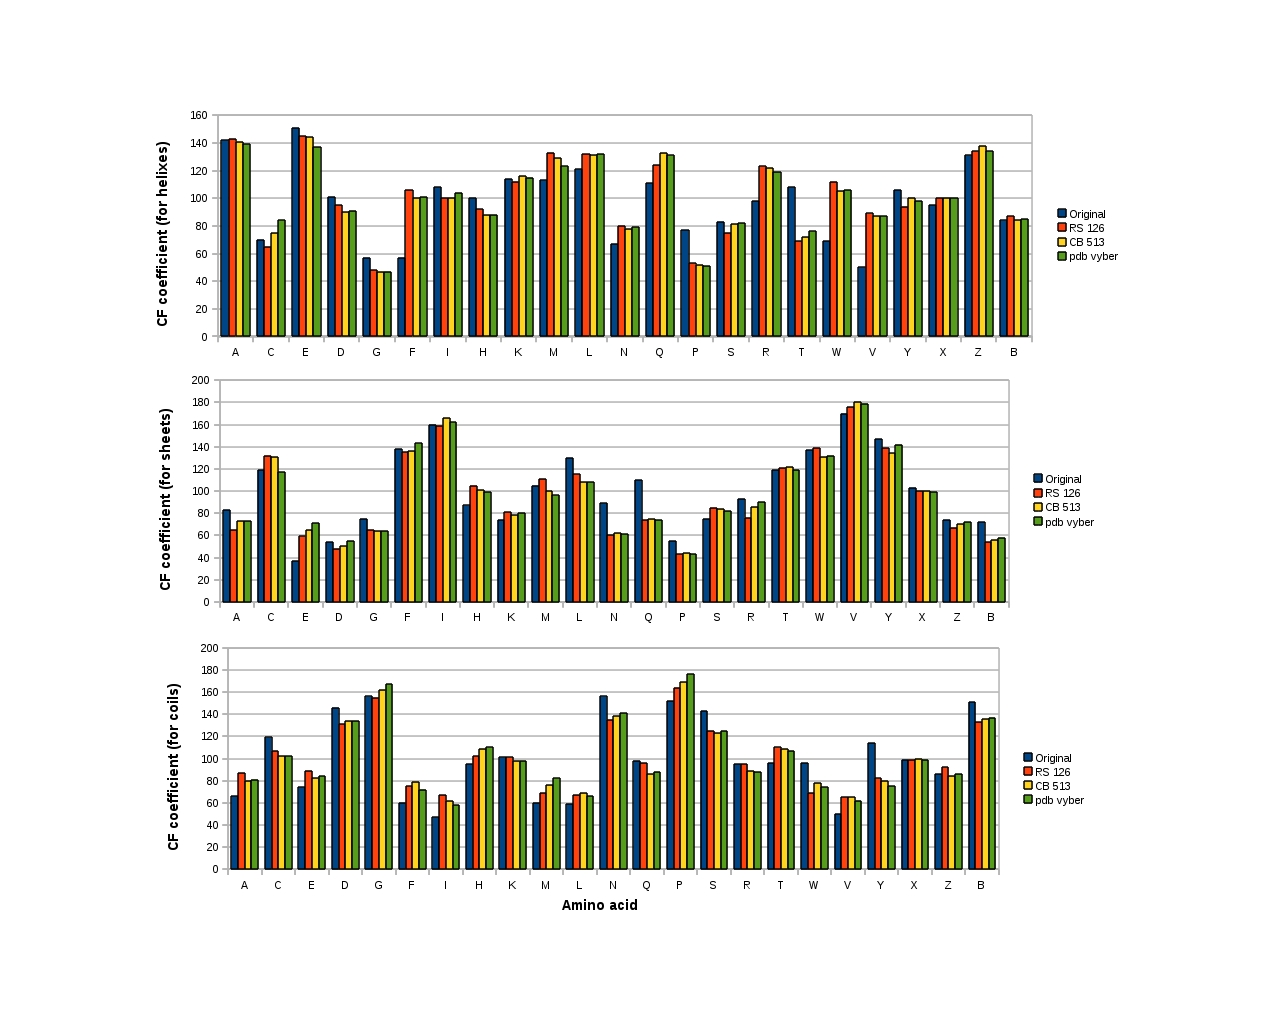
\includegraphics{pics/cf_comparision.jpg}}
  \caption{meeeh}
  \label{obr:cf_comparision}
  \end{center}
\end{figure}



\chapter{V�sledky experimentov}
% tabulky vysledkov experimentov

